\documentclass{article}
\usepackage{natbib}
\usepackage{hyperref}
\usepackage{graphicx}
\usepackage{subcaption}
\usepackage{amsmath}
\bibliographystyle{apalike}

\title{Testing Efficacy; Insights from a Simple Epidemic Model }

\begin{document}
\maketitle

% %%%%%%%
\section{Introduction}

- Why non-random testing/testing-tracing-isolation (TTI) is more efficent in controling an epidemic event?
- Literature reviwe, evidences of efficacy of TTI
- Simple ODE models provide useful insights (some classic examples, Kermack-Makendric,...)
Historically, Ronald Ross (I think) developed a series of mathematical models to study the spread of malaria and implementation of control. His work contributed to the modern theory of the control of
infectious disease (ref: Ross R. The Prevention of Malaria, 2nd edn. London: Murray, 1911).


- Covid-19 and chalanges, questions to be addressed with a simple model.
This study provides a framework/platform to study a pandamic in a population with a determinstic system of differential equations with testing mechinisms and isolation. 

- Our work; we developed a deterministic compartmental model which incorporates testing strategies and isolation mechanism. 
- The basic reproduction number was derived analytically as a threshold of the dynamics. 
- Our simulation shows ...

% %%%%%%%
\section{Literature Review}

\subsection{Explicit models of TTI (trace/test/isolate) based on network or agent-based models}
\citep{endo2020implication} [Ali: It seems to me that this is just a statistical model to estimate the parent-offspring of an infected index, not sure if it fits into agent-based group!] Used simulation on a branching process model to assess the forward and backward contact tracing efficiency. Assuming a negative-binomial branching process with a mean R, reproduction number, and overdispersion parameter k, the mean total number of generation G3 and averted G3 are estimated. The effectiveness of TTI is defined as the ratio of averted to the mean.

\citep{jenness2020modeling} developed a network-based transmission model for SARS-CoV-2 on the Diamond Princess outbreak to characterize transmission dynamics and to estimate the epidemiological impact of outbreak control and prevention measures. 

\citep{elbanna2020entry} [seems similar to MacPan model!]

\citep{de2020influenza} Was discussed in the Math 747 
SEIR Asymptomatic and symptomatic $I_1, I_2$. Used linear chain trick 
Stringency index as a control force lowering $\beta$.

\citep{rice2020effect} Effect of school closures on mortality. Reproduce Report 9 results by spatial agent based CovidSim. 
% %%%%%%%
\subsection{Models of repeated random testing of isolated populations}
\cite{bergstrom2020frequency}
(1) Model, assumptions: They developed a function, namely expected exposure $E(C,\tau)$, to approximate trade-offs between the frequency of testing, n, the sensitivity of testing, q, and the delay between
testing and results, d. This function is explicitly derived and was connected the effective reproduction number $R=R_0 S$, where $S$ is the proportion of population susceptible.
assumption that transmission rates are a step function: individuals who
have COVID go from non-infectious to fully infectious instantaneously,
and remain fully infectious until they are no longer able to transmit disease. Test sensitivity takes the same form over the course of infection.
More sophisticated models could allow varying infectiousness and varying
sensitivity over time, as in 
\citep{larremore2020test}.

\citep{lopman2020model} Used a Deterministic SEIR model, incorporated TTI, applicable to a university setting. They assumed a fairly high reproductive number that is not reduced through social
distancing measures. They found that community-introduction of SARS-CoV-2 infection onto campus can be
relatively controlled with effective testing, isolation, contract tracing and quarantine.

\citep{tuite2020mathematical} used an age-structured compartmental model of COVID-19 transmission in the population of Ontario, Canada. We compared a base case with limited testing, isolation and quarantine to different scenarios. 
% %%%%%%%
\subsection{Other maybe-related works}
\citep{arino2020simple} developed a SLIAR compartmental model to study the spread of an epidemic, specifically COVID-19, in a population. The model incorporates an Erlang distribution of times of sojourn in incubating, symptomatically and asymptomatically infectious compartments. Basic reproduction number is derived. Also, sensitivity analysis with respect to the underlying parameters for the following two outputs was carried out; (i) the number of observable cases during the course of the epidemic and at the peak, and (ii) the timing of the peak of the outbreak. Sensitivity analysis is performed using the R package multisensi.

\citep{ruszkiewicz2020diagnosis} novel with-in-a-minute breath testing with 80\% accuracy. 

% %%%%%%%
\section{Method}
\begin{itemize}
\item $\Lambda$: force of infection defined as $$\Lambda=\beta \frac{(I_u+\eta_w I_n+\eta_w I_p+ \eta_t I_t)}{N_0},$$ where $\beta$ is transmission rate, $\eta_w$ and $\eta_t$ are the isolation parameters for awaiting and reported individuals, respectively. We assume that $\eta_t \leq \eta_w$, i.e., the awaiting individuals for test results have a higher transmission probability than the reported individuals.
\item $\omega$: the rate of onward flow from the awaiting positive compartment, $p$, to reported/tested compartment, $\rho$, or from awaiting negative compartment, $n$, back to $u$.  It has units of 1/time.
\item $\gamma$: recovery rate (1/time).
\item $\rho$: per capita testing intensity across the whole population (1/time).
\item $W$: weighted number of people available for tests, defined as $W = W_S S_u + W_I I_u + W_R R_u$.
\item $\sigma$: scaling parameter for testing defined as $\sigma = \frac{\rho N_0}{W}$.
\item $F_Z$: Weighted testing rate defined as $F_Z=\sigma W_Z$. That is, $F_S = \sigma W_S$, $F_I=\sigma W_I$ and $F_R = \sigma W_R$.
\end{itemize}

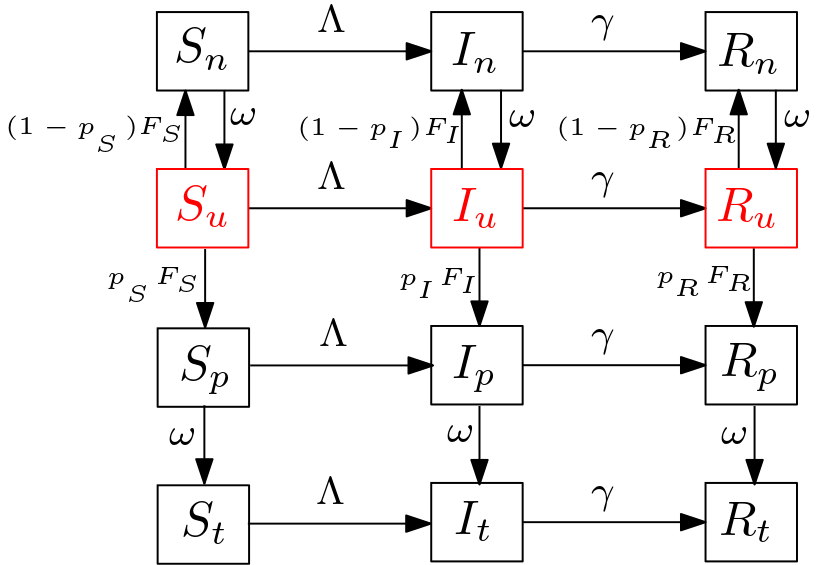
\includegraphics[width=\linewidth]{./pix/sir_comp.png}

The model is

\begin{align}
\label{model}
 d S_u/dt &= -\Lambda S_u - F_S S_u + \omega S_n \\
 d S_n/dt &= -\Lambda S_n + (1-p_S) F_S S_u - \omega S_n \\
 d S_p/dt &= -\Lambda S_p + p_S F_S S_u - \omega S_p \\
 d S_t/dt &= -\Lambda S_t + \omega S_p \\
 d I_u/dt &= \Lambda S_u - F_I I_u + \omega I_n  - \gamma I_u  \\
 d I_n/dt &= \Lambda S_n + (1-p_I) F_I I_u - \omega I_n -\gamma I_n \\
 d I_p/dt &= \Lambda S_p + p_I F_I I_u - \omega I_p -\gamma I_p \\
 d I_t/dt &= \Lambda S_t + \omega I_p - \gamma I_t  \\
 d R_u/dt &= \gamma I_u - F_R R_u + \omega R_n \\
 d R_n/dt &= \gamma I_n + (1-p_R) F_R R_u - \omega R_n  \\
 d R_p/dt &= \gamma I_p + p_R F_R R_u  - \omega R_p  \\
 d R_t/dt&= \gamma I_t + \omega R_p  \\
 dN/dt &= \omega (S_n + I_n + R_n)   \\
 dP/dt &= \omega(I_p + R_p).
\end{align}

- Assumptions of this model:
-why not bith and death are included?

% %%%%%%%
\section{Results}


% %%%%%%%
\section{Discussion}

- May be something about the testing rate/intensity, now the per capita testing intensity is very low ($\rho \approx 0$). In near future new test kits may be widely accessible, our model provide insights in this case (what are those?)

- "delay negative results" result


% %%%%%%%
\bibliography{SIRlibrary.bib}

\end{document}
